\chapter{Introduction}
\label{chapter:intro}
\pagestyle{mainmatter}
\pagenumbering{arabic}

\epigraph{\small\itshape ``Progress in science depends on new techniques, new discoveries and new ideas, probably in that order.''}{\small\textit{---Sidney Brenner}}

\begin{figure}[ht!]
\centering
\begingroup
\etocstandardlines
%\renewcommand{\etocbkgcolorcmd}{\color{lightgray}}
\renewcommand{\etocbelowtocskip}{0pt\relax}
\fboxsep1ex
\etocframedstyle [1]{\fbox{\makebox[.4\linewidth]{\etocfontminusone
Contents}}}
\localtableofcontents
\endgroup
\end{figure}

\clearpage

Understanding the human brain is one of the most significant challenges of the 21st century. The human brain is arguably the most complex  organs of the human body, which performs a wide range of cognitive functions: from visual recognition to language understanding, speech, social interaction, and executive control. Pathologies of the brain are perhaps on of the biggest challenges for medicine today. Medical interventions and drugs for major infectious diseases are available today, and individuals can expect to live up to the mid 80s and even into their 90s. Yet, we still do not have a good grasp over most mental pathologies: Parkinson's, Alzheimer's, dementia, epilepsy to name a few. This is despite the fact that someone today who lives into their mid 80s has a 50\% chance of contracting Alzheimer's~\citep{alzheimer20162016}.

Our current understanding of the brain is a result of decades of concerted efforts across multiple disciplines ranging from molecular biology, genetics, physiology, cognitive and behavioral neuroscience, to statistics, computer science, and data science. A relatively new subfield here is brain imaging, also known as neuroimaging. Brain imaging refer to a set of technologies where a snapshot of the brain is taken to measure either the anatomy or various aspects of function. The grand vision is to be deploy them in hospitals to help diagnosis, in surgeries, in \acp{BCI}, or in research for neuroscientists to better understand the brain. 
In this thesis, we will focus our attention on measuring the electric currents and/or corresponding magnetic field from the brain, using electroencephalography, magnetoencephalography, and local field potentials. 
These methods have the property of possessing a high temporal resolution, which is particularly useful for extracting the temporal dynamics of brain signals.

In this manuscript, I will describe several methodological advances that we achieved in brain imaging using our expertise in machine learning and open source software. In the forthcoming sections, I will first describe the context surrounding the thesis. After a brief introduction to the field of electrophysiology, I will delve into how the field has been shaped in recent years by the reproducibility crisis, and how data sharing is going to help alleviate this problem to a large extent. However, the rise of data sharing and large sample sizes makes it difficult to still rely on manual data analysis which does not scale and is not reproducible. To cope with this challenge, we must start relying on automated and data-driven methods for discovering new effects. To this effect, I will introduce two new algorithms \emph{autoreject} and \emph{alphacsc}. This is followed by a refresher on background material that might be useful to refer to when reading the thesis. The chapter ends with the contributions of this thesis and the list of papers published during the PhD.
 
%\section{Modern brain imaging}
%Brain imaging tools today can be placed along three axes: their temporal resolution, their spatial resolution, and the level to which they are invasive.

\section{Electrophysiology}

\begin{figure}[htb]
\begin{center}
   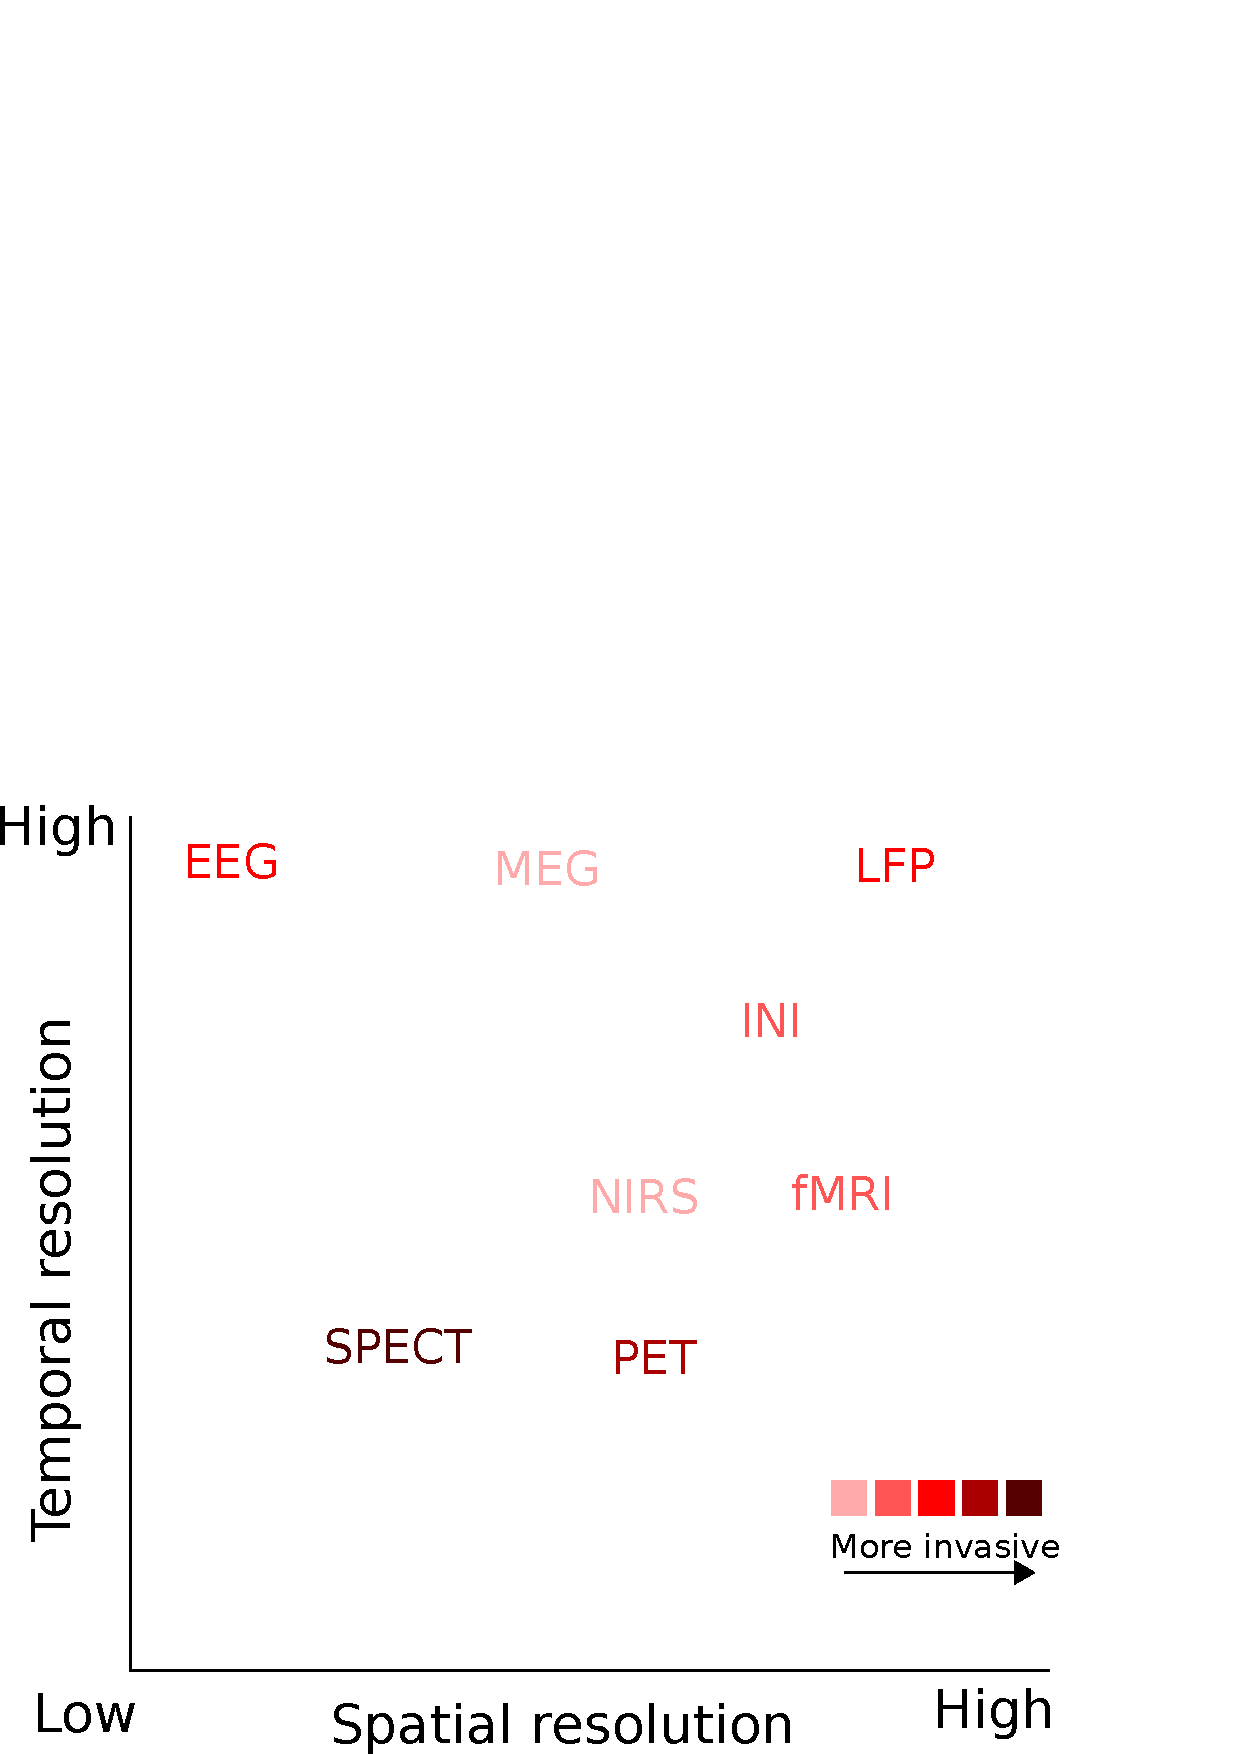
\includegraphics[width=0.5\linewidth]{figures/neuroimaging_methods.pdf}
\end{center}
   \caption[Various neuroimaging methods differ in terms of the information they measure.]{Various neuroimaging methods differ in terms of the information they measure. MEG=magnetoencephalography, EEG=electroencephalography, NIRS=near-infrared spectroscopy, PET=positron emission tomography, SPECT=single photon emission tomography, and INI=Inverse imaging, a method to speed up acquisition of fMRI images, ECoG=Electrocorticography, LFP=Local Field Potential.}
   \label{fig:neuroimaging_methods}
\end{figure}

The study of electrical properties of the biological cells and tissues is known as electrophysiology. 
Biological tissues have electrical properties due to the presence of ions. Just as we can measure voltages in electrical appliances, it is possible also to measure these voltages in living tissues. 
These modalities have the advantage of directly measuring the brain activity, as opposed to an indirect measure, which is for example the case in \ac{fMRI}.
Brain imaging techniques are characterized by their temporal and spatial resolution, \textit{i.e.,} the time scale at which it can measure brain activity, and also the accuracy of localizing the source of the activity. Figure~\ref{fig:neuroimaging_methods} summarizes different neuroimaging methods with respect to their temporal and spatial resolution. In the case of \ac{fMRI}, as it measures the blood flow which is a response to neural activity and slowly changing, its temporal resolution cannot be high. 

There are a number of modalities to measure the electrical potentials in the human body, the most well-known being perhaps \ac{ECG} which is used to measure the heart beats. However, in our work, we will focus on only three which are relevant for studying the brain. Each of these methods produces a multivariate time series.

\paragraph{Electroencephalography: } \Ac{EEG} is a portable and non-invasive measurement modality that is frequently used in the context of \acp{BCI}. 
In electroencephalography, an array of electrodes on an \ac{EEG} cap is placed on the scalp to measure the voltages with respect to a reference electrode. 
The voltage it measures is not the result of a single neuron but instead a summed potential of populations of thousands of neurons. It has a high temporal resolution (in the order of \emph{ms}), however the spatial resolution is not so high as the skull smears the signal.

\paragraph{Magnetoencephalography: } Any electric current is associated with magnetic fields as a consequence of Maxwell's theory. 
Therefore, the brain generates tiny magnetic fields which  wrap around the currents according to Maxwell's right hand thumb rule. The flux is tiny ($\sim10^{-12}T$) compared to the earth's magnetic field ($\sim10^{-4}T$), and to measure it one would need very sensitive electronics and heavy noise cancellation. The measurement itself is done in a magnetically shielded room made of three layers of metals. 
The sensors are superconducting coils which capture the magnetic flux. They are immersed in liquid helium cooled to very low temperatures, so as to lower any loss in signal due to resistance. A typical device contains two types of sensors: gradiometers and magnetometers. While the magnetometer measures the absolute magnitude of magnetic field, the gradiometer measures derivative of the field. \Ac{MEG} has the advantage that the skull does not deteriorate the signal quality as in \ac{EEG}.

\paragraph{\Ac{LFP}}
The Local Field Potential is the electric potential that is recorded in the extracellular space of the brain tissue. In contrast to \ac{EEG}, \ac{LFP} are recorded in depth, from within the cortical tissue and can therefore measure more localized populations of neurons. Small intracerebral electrodes are typically used to measure these potentials as opposed to large surface electrodes used in \ac{EEG}.
